%==========================================================================
% CAPÍTULO 4 — DESENVOLVIMENTO
%==========================================================================
\chapter{Desenvolvimento}
\label{chap:desenvolvimento}

% ------------------------------------------------------------------
% Nota sobre Data Augmentation
% ------------------------------------------------------------------
\section*{Nota sobre Contagem de Imagens}
\addcontentsline{toc}{section}{Nota sobre Contagem de Imagens}

Durante o treino na plataforma Roboflow Train, a plataforma aplica
automaticamente técnicas de \textit{data augmentation} (rotações,
espelhos, variações de brilho e contraste, entre outras) sobre as
imagens anotadas. Os valores de contagem de imagens reportados no
painel do Roboflow referem-se sempre ao total \textbf{após
augmentation}, e não ao número de imagens base originalmente anotadas.

A Tabela~\ref{tab:datasets_aug} resume a composição de cada versão
do dataset, distinguindo as contagens base das contagens pós-augmentation.

\begin{table}[H]
  \centering
  \caption{Composição dos datasets por modelo (imagens base vs.\
           após \textit{data augmentation})}
  \label{tab:datasets_aug}
  \begin{tabularx}{\textwidth}{l c c c X}
    \toprule
    \textbf{Modelo} & \textbf{Base SVY-2} & \textbf{Base Palmela}
                    & \textbf{Base total} & \textbf{Após augmentation (Roboflow)} \\
    \midrule
    Modelo 1 & 300 & 0   & 300  & $\approx$775 \\
    Modelo 2 & 300 & 100 & 400  & 772 \\
    Modelo 3 & 300 & 100+ & 400+ & 938 \\
    \bottomrule
  \end{tabularx}
\end{table}

% ------------------------------------------------------------------
\section{Modelo 1 — \textit{Segmentation-Vineyard-2} (fase de validação técnica)}
% ------------------------------------------------------------------

\subsection{Caracterização do Dataset}

O primeiro modelo foi desenvolvido com base no dataset público
\textbf{Segmentation-Vineyard-2}~\cite{vinya2024segvineyard}, disponível na
plataforma Roboflow Universe e de origem espanhola. Este dataset continha
originalmente apenas anotações de \texttt{sarmento} e \texttt{tronco} —
não incluía qualquer anotação de gomos.

A contribuição deste estágio consistiu em anotar manualmente os
gomos em cada uma das 300 imagens do dataset, acrescentando a classe
\texttt{gomo} ao conjunto de etiquetas existente. O Modelo~1 passou assim
a ter três classes: \texttt{gomo}, \texttt{sarmento} e \texttt{tronco}.
O dataset foi dividido na plataforma Roboflow nas proporções
70\% treino / 20\% validação / 10\% teste. Após a aplicação de
\textit{data augmentation} pelo Roboflow, o conjunto de treino
atingiu aproximadamente 775 imagens.

O processo de desenvolvimento do Modelo~1 serviu como etapa de validação
da \textit{pipeline} técnica e permitiu confirmar a viabilidade do fluxo
completo de anotação, treino e inferência antes de introduzir as imagens
de Palmela, de maior complexidade.

\subsection{Refinamento das Etiquetas}

Após uma inspeção visual inicial do \textbf{Segmentation-Vineyard-2}, foram identificadas
algumas inconsistências nas anotações de \texttt{sarmento} e \texttt{tronco}
— \textit{bounding boxes} excessivamente largas ou com sobreposição não
intencional. Procedeu-se ao refinamento manual de parte dessas anotações,
em simultâneo com a adição das anotações de \texttt{gomo}.

\subsection{Observações Qualitativas}

A inferência sobre imagens do conjunto de teste revelou que o modelo
identifica corretamente os sarmentos com elevada confiança (até 97\%)
e os troncos com boa confiança (acima de 83\%). As métricas formais
deste modelo foram obtidas apenas na versão do Roboflow correspondente
ao Modelo~2 (que utilizou o mesmo dataset base acrescido das imagens de
Palmela), dado que ambas as versões foram treinadas numa única sessão
sequencial na plataforma.

% ------------------------------------------------------------------
\section{Modelo 2 — SVY-2 + Palmela (400 imagens base)}
\label{sec:modelo2}
% ------------------------------------------------------------------

\subsection{Justificação e Contexto}

O desenvolvimento do segundo modelo representa o núcleo do trabalho prático
deste estágio. A motivação para a criação de um novo dataset, em vez de
reutilizar integralmente o dataset espanhol, reside na diferença substancial
entre as condições das imagens disponíveis publicamente e as condições reais
de operação de um robô de poda nas vinhas portuguesas.

As imagens do \textbf{Segmentation-Vineyard-2} foram, na sua maioria, captadas em condições
controladas ou com planos de fundo limpos. Em contrapartida, um robô real
que percorra as vinhas de Palmela capturará cenas com:

\begin{itemize}
  \item Múltiplas videiras visíveis em simultâneo (primeiro e segundo planos);
  \item Arames de suporte, postes e outros elementos de infraestrutura;
  \item Reflexos de luz solar e variações abruptas de contraste;
  \item Sarmentos de diferentes espessuras e comprimentos que se cruzam
    e sobrepõem no campo visual.
\end{itemize}

É precisamente esta realidade que o Modelo~2 pretende capturar.

\subsection{Processo de Captação de Vídeo}

Os vídeos utilizados para construir o dataset de Palmela foram captados
durante uma visita às vinhas da região, realizada em março de 2026. A
captação foi efetuada com câmera de smartphone em modo vídeo, percorrendo
as fileiras de videiras a pé, de forma a simular o deslocamento de um
robô agrícola.

Para cobrir diferentes perspetivas e condições de iluminação, foram
realizadas passagens ao longo de várias filas em diferentes horas do dia.
A taxa de captura foi configurada em \textbf{2 frames por segundo} no
Roboflow, o que corresponde a uma amostragem suficiente para capturar a
diversidade visual sem criar um número excessivo de frames redundantes.

\subsection{Importação e Extração de Frames no Roboflow}

Os ficheiros de vídeo (formato \texttt{.mp4}) foram importados diretamente
para o projeto no Roboflow. A plataforma realiza automaticamente a extração
dos frames à taxa configurada e apresenta-os sequencialmente para anotação.
Esta funcionalidade reduziu significativamente o tempo de pré-processamento
manual dos dados.

\subsection{Evolução da Estratégia de Anotação}

Ao longo das sessões de anotação do dataset de Palmela, a estratégia foi
sendo refinada com base nas dificuldades encontradas. A decisão de incluir
as classes \texttt{tronco} e \texttt{objeto} surgiu após as primeiras experiências
de treino revelarem que o modelo confundia estes elementos com sarmentos e
gomos.

A inclusão dos sarmentos como classe própria — e não apenas como
contexto — foi igualmente determinante. Ao delimitar os sarmentos, o modelo
adquire um guia estrutural que facilita a localização dos gomos, que crescem
ao longo dos sarmentos em posições relativamente regulares.

\subsection{Dificuldades Específicas e Decisões Tomadas}

\paragraph{Densidade de instâncias por imagem.}
Cada imagem das vinhas de Palmela pode conter dezenas de gomos visíveis.
A política de anotação adoptada foi a de marcar o máximo de gomos
identificáveis em cada imagem. Esta decisão baseia-se numa característica
biológica favorável: os gomos crescem em posições regulares e previsíveis ao
longo dos sarmentos, pelo que os seus locais de inserção são reconhecíveis
mesmo a distância ou em condições de visibilidade parcial. Omitir gomos
identificáveis introduziria falsos negativos sistemáticos no treino,
prejudicando a capacidade de \textit{recall} do modelo.

\paragraph{Ambiguidade de fronteiras entre classes.}
Em certas imagens, a distinção entre um sarmento em primeiro plano e um
tronco em segundo plano é subjetiva. Foi adotada a regra de que a classe é
determinada pela posição relativa ao plano focal principal: o elemento mais
próximo da câmera é classificado pelo seu tipo real.

\paragraph{Gomos muito pequenos.}
Em imagens captadas a maior distância, os gomos aparecem com dimensões
inferiores a 15$\times$15~px. Estes casos foram anotados quando identificáveis,
mas reconhece-se que o modelo terá maior dificuldade em detetá-los.

\subsection{Estado da Anotação e Métricas}

Até à data de elaboração deste relatório, foram anotadas aproximadamente
100 imagens provenientes das vinhas de Palmela, que foram
combinadas com as 300 imagens do Segmentation-Vineyard-2 para compor o
dataset do Modelo~2 (400 imagens base no total). Após a aplicação de
\textit{data augmentation} pelo Roboflow, o conjunto de treino atingiu
772 imagens, divididas nas proporções 70\% treino / 20\% validação /
10\% teste.

A Tabela~\ref{tab:resultados_m2_dev} apresenta as métricas obtidas no
conjunto de validação.

\begin{table}[H]
  \centering
  \caption{Métricas do Modelo 2 no conjunto de validação (Roboflow Train)}
  \label{tab:resultados_m2_dev}
  \begin{tabular}{lc}
    \toprule
    \textbf{Métrica}   & \textbf{Valor} \\
    \midrule
    mAP@50             & 48,8\% \\
    Precisão           & 54,3\% \\
    Recall             & 52,7\% \\
    F1-Score           & 53,5\% \\
    \bottomrule
  \end{tabular}
\end{table}

Os resultados são moderados mas coerentes com a natureza do Modelo~2:
dataset de domínio misto (espanhol + português), quatro classes com
densidades de instâncias muito distintas, e uma classe (\texttt{gomo})
completamente nova relativamente ao dataset base. A precisão de 54,3\%
e o recall de 52,7\% equilibrados indicam que o modelo distribui as
dificuldades de forma homogénea, sem enviesamento sistemático.

O dataset encontra-se versionado no Roboflow, permitindo reprodutibilidade
dos treinos e rastreabilidade das alterações de anotação.

% ------------------------------------------------------------------
\section{Modelo 3 — Dataset Expandido (400+ imagens base, 938 augmentadas)}
\label{sec:modelo3}
% ------------------------------------------------------------------

\subsection{Contexto e Motivação}

Com base nos resultados do Modelo~2 e na análise qualitativa das
inferências, foi construída uma terceira versão do dataset com imagens
de Palmela adicionais. O objetivo foi avaliar se o aumento do volume de
dados resultaria numa melhoria das métricas, em particular no Recall da
classe \texttt{gomo}.

\subsection{Composição do Dataset e Resultados}

O dataset do Modelo~3 foi gerado em 17 de junho de 2026, com um total de
938 imagens após augmentation. A Tabela~\ref{tab:resultados_m3_dev}
resume as métricas obtidas no conjunto de validação.

\begin{table}[H]
  \centering
  \caption{Métricas do Modelo 3 no conjunto de validação (Roboflow Train)}
  \label{tab:resultados_m3_dev}
  \begin{tabular}{lc}
    \toprule
    \textbf{Métrica}   & \textbf{Valor} \\
    \midrule
    mAP@50             & 43,7\% \\
    Precisão           & 57,3\% \\
    Recall             & 40,5\% \\
    F1-Score           & 47,4\% \\
    \bottomrule
  \end{tabular}
\end{table}

A Figura~\ref{fig:resultado_m3} mostra uma inferência do Modelo~3 sobre
uma imagem das vinhas de Palmela, com \textit{confidence threshold} de 16\%.

\begin{figure}[H]
  \centering
  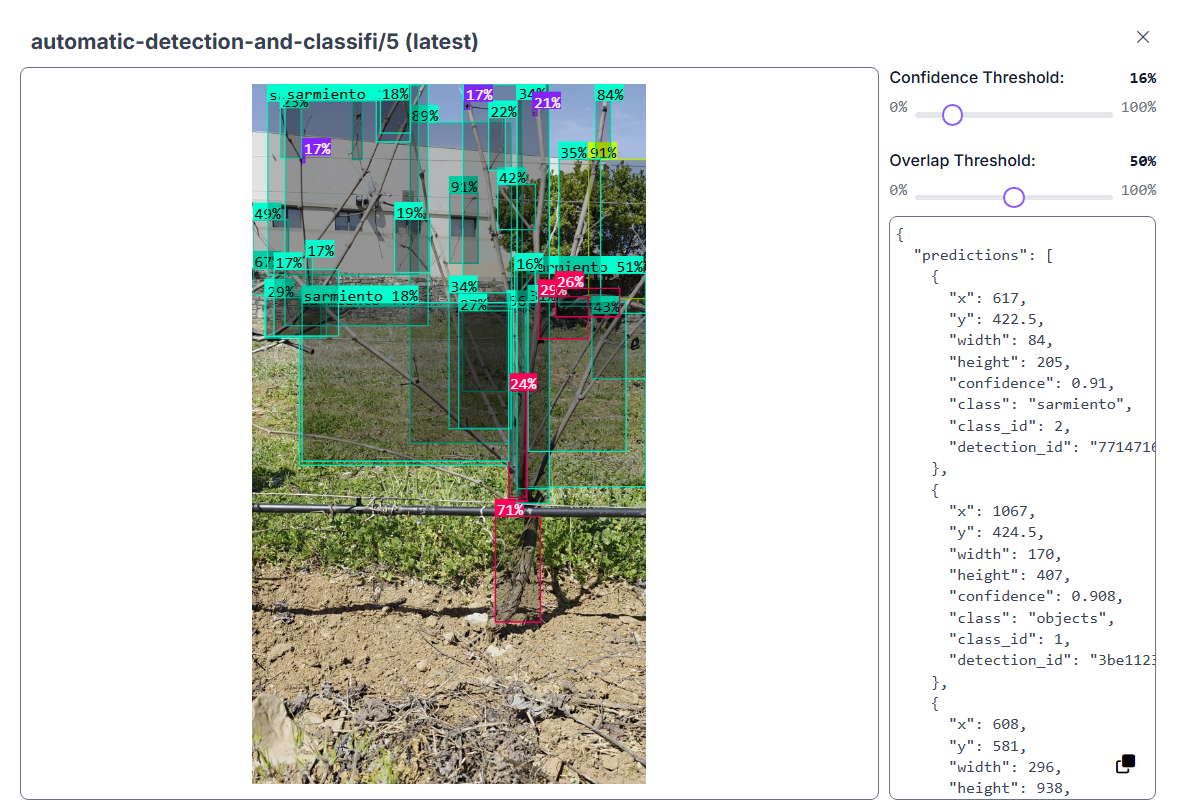
\includegraphics[width=0.85\textwidth]{imagens/resultado_v3.png}
  \caption{Inferência do Modelo~3 sobre imagem das vinhas de Palmela
           (\textit{threshold} = 16\%). Sarmentos (ciano), gomos (roxo),
           objetos (vermelho). Os sarmentos atingem confiança até 91\%;
           os gomos surgem apenas com confiança de 16--26\%, indicando
           que a classe está a ser aprendida mas requer mais dados.}
  \label{fig:resultado_m3}
\end{figure}

\subsection{Análise dos Resultados do Modelo 3}

A comparação entre o Modelo~2 (mAP@50 = 48,8\%) e o Modelo~3
(mAP@50 = 43,7\%) revela uma descida ligeira nas métricas globais, que
se explica pelo aumento da complexidade do dataset — mais imagens de
Palmela com maior densidade de instâncias e mais variação visual. Não
obstante, a Precisão subiu de 54,3\% para 57,3\%, o que indica menos
falsos positivos. O Recall de 40,5\% reflete a dificuldade em detetar
gomos com confiança suficiente para ultrapassar o limiar de 50\%.

A análise da inferência (Figura~\ref{fig:resultado_m3}) revela que:
\begin{itemize}
  \item Os sarmentos são detetados com elevada confiança (até 91\%);
  \item Um objeto (estaca/poste) é detetado corretamente com 71\% de confiança;
  \item Os gomos surgem com confiança de 16--26\%, indicando que o modelo
    está a aprender a classe, mas o volume de dados ainda é insuficiente
    para calibrar a confiança neste nível.
\end{itemize}

Este comportamento é esperado para uma classe de pequena dimensão com
elevada variabilidade intra-classe e volume de dados limitado.

% ------------------------------------------------------------------
\section{Considerações sobre a Complexidade do Problema}
% ------------------------------------------------------------------

A experiência acumulada durante o estágio permite afirmar que a tarefa de
deteção de gomos em cenas reais de vinha, com a complexidade visual observada
nas imagens de Palmela, é um problema que excede o que pode ser
resolvido satisfatoriamente num único semestre de trabalho. As razões são
múltiplas:

\begin{enumerate}
  \item Volume de dados: modelos de deteção de objetos em cenas
    complexas tipicamente requerem milhares de imagens anotadas por classe.
    Com 100 imagens de Palmela (400+ no total com as espanholas), o modelo
    está limitado na sua capacidade de generalização.

  \item Complexidade de anotação: a anotação de imagens com grande
    densidade de instâncias é demorada e exige consistência. A taxa de
    anotação estimada é de 15--25 imagens por hora para imagens de alta
    densidade.

  \item Variabilidade do domínio: as condições de iluminação,
    fenologia e morfologia variam significativamente entre épocas do ano,
    o que implica a necessidade de múltiplas rondas de captura.

  \item Otimização do modelo: a escolha dos hiperparâmetros e das
    técnicas de \textit{data augmentation} adequadas ao domínio específico
    requer múltiplas iterações de treino e avaliação.
\end{enumerate}

Não obstante, o trabalho desenvolvido até ao momento estabelece uma base
metodológica sólida e fornece uma avaliação realista dos desafios envolvidos,
constituindo um ponto de partida valioso para projetos de continuação.
